\chapter{Results}
A watermarked audio sample has been recorded\footnote{The recording was made with Samsung Tab S6 Lite. The audio watermark, however, is emitted from a Samsung S20+ 5G.} and then analyzed with the script listed in Appendix \ref{code}. Here the results are reported and discussed.
\section{Analysis of the result of a watermarked audio recording.}
As a first step, let's analyze the spectrum and magnitude of the "raw" signal.
In figure \ref{fig:raw_signal} is reported the spectrum of the signal on the left (\ref{fftraw}) and the plain signal on the right (\ref{rawsig}). The audio sample comprises a sentence ("example of watermarked audio") that has been marked using the previously described application. The watermark is set to a simple string ('ciao') and a GPS location, both encrypted with the methods previously explained, using as key the string \textit{"AWESOMEKEY"}.
\begin{figure}[H]
    \centering
    \begin{subfigure}{0.48\textwidth}
    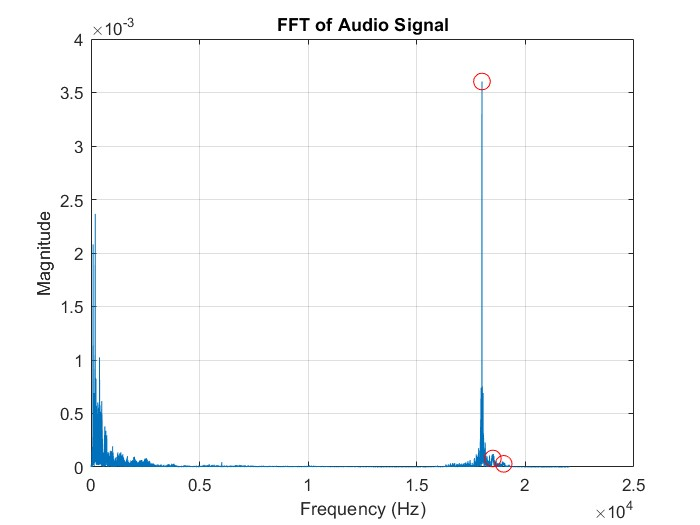
\includegraphics[width=\textwidth]{LiveAudioWatermarking/images/FFT_raw.jpg}
    \caption{}
    \label{fftraw}
    \end{subfigure}%
    \hfill
     \begin{subfigure}{0.48\textwidth}
    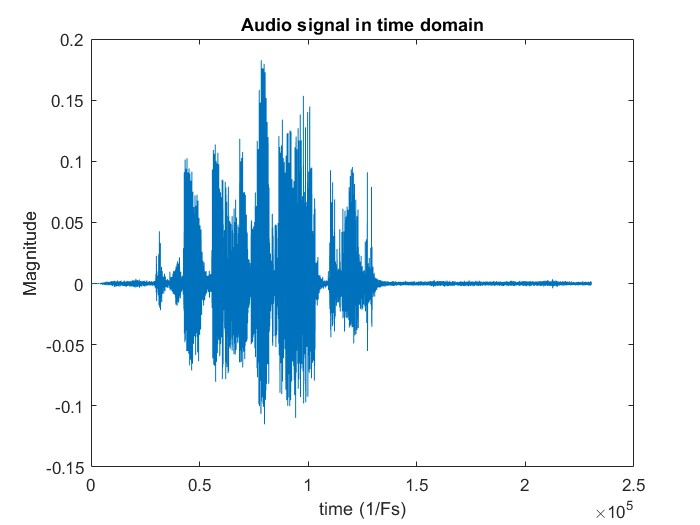
\includegraphics[width=\textwidth]{LiveAudioWatermarking/images/sig_td_raw.jpg}
    \caption{}
    \label{rawsig}
    \end{subfigure}
    \caption{Unprocessed audio sample}
    \label{fig:raw_signal}
\end{figure}
It can be observed from the figure that there is some content at the desired frequency, indicating that the watermark has been successfully embedded into the audio file.
The result of the applied band-pass filter is shown in figure \ref{fig:filtered_signal}. The filtered data contains only the audio watermark. When listening to the processed signal, no noise can be heard.


\begin{figure}[H]
    \centering
    \begin{subfigure}{0.48\textwidth}
    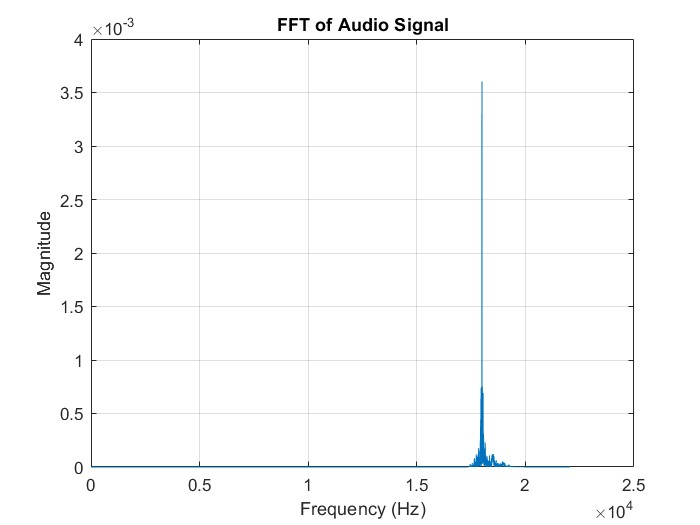
\includegraphics[width=\textwidth]{LiveAudioWatermarking/images/FFT_filtered.jpg}
    \caption{}
    \label{}
    \end{subfigure}%
    \hfill
     \begin{subfigure}{0.48\textwidth}
    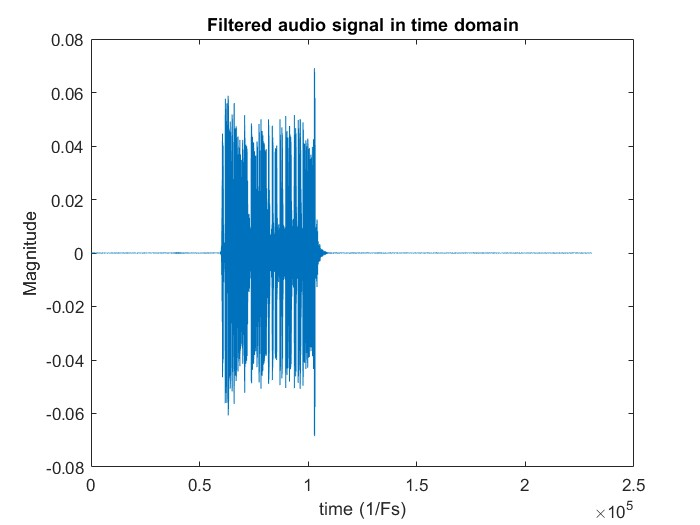
\includegraphics[width=\textwidth]{LiveAudioWatermarking/images/sign_td_filt.jpg}
    \caption{}
    \label{}
    \end{subfigure}
    \caption{pre-processed audio sample}
    \label{fig:filtered_signal}
\end{figure}

The subsequent phase involves determining the positions of both the start and stop bits. For this purpose, cross-correlation analysis was conducted using the 'xcorr' command in Matlab between a tone generated in the script and the pre-processed audio track. The results of these analyses are displayed in figure \ref{fig:tonesearch}. The red circle indicates the index (more precisely the \textit{lag} with respect the start of the audio sample) at which the tone begins.

\begin{figure}[H]
    \centering
    \begin{subfigure}{0.48\textwidth}
    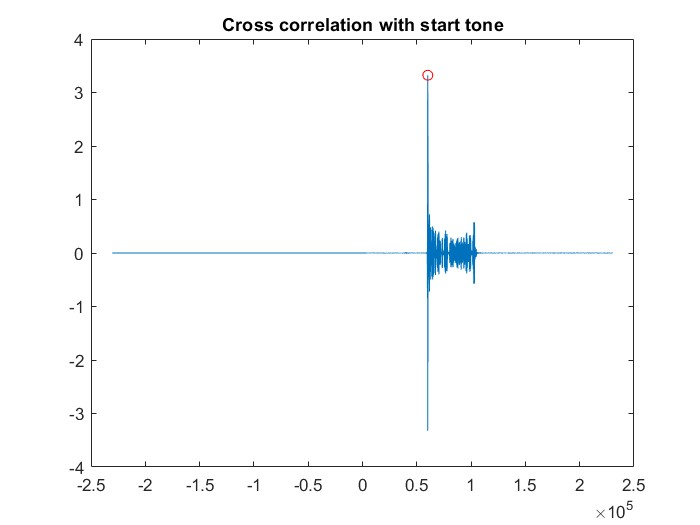
\includegraphics[width=\textwidth]{LiveAudioWatermarking/images/cross_start.jpg}
    \caption{}
    \label{}
    \end{subfigure}%
    \hfill
     \begin{subfigure}{0.48\textwidth}
    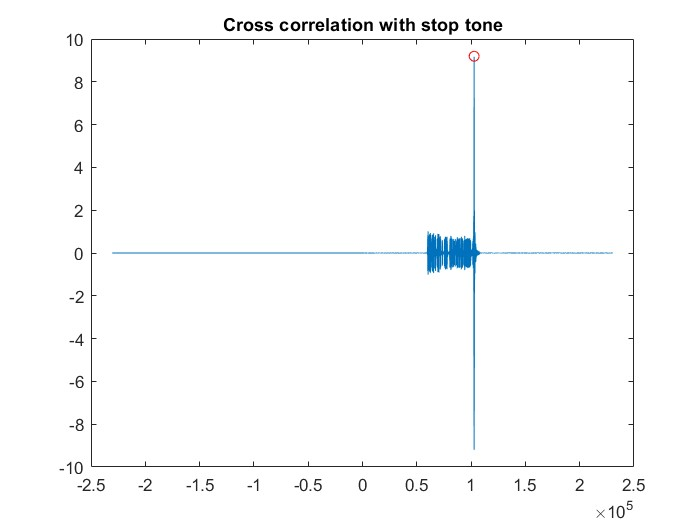
\includegraphics[width=\textwidth]{LiveAudioWatermarking/images/cross_stop.jpg}
    \caption{}
    \label{}
    \end{subfigure}
    \caption{cross correlation results}
    \label{fig:tonesearch}
\end{figure}

After identifying these tones, we can deduce the length of the watermark. By knowing the duration of the tone, we can extract segments for further analysis using additional signal processing techniques. a representation of the segments can be found in figure \ref{fig:segments}
\begin{figure}[H]
    \centering
    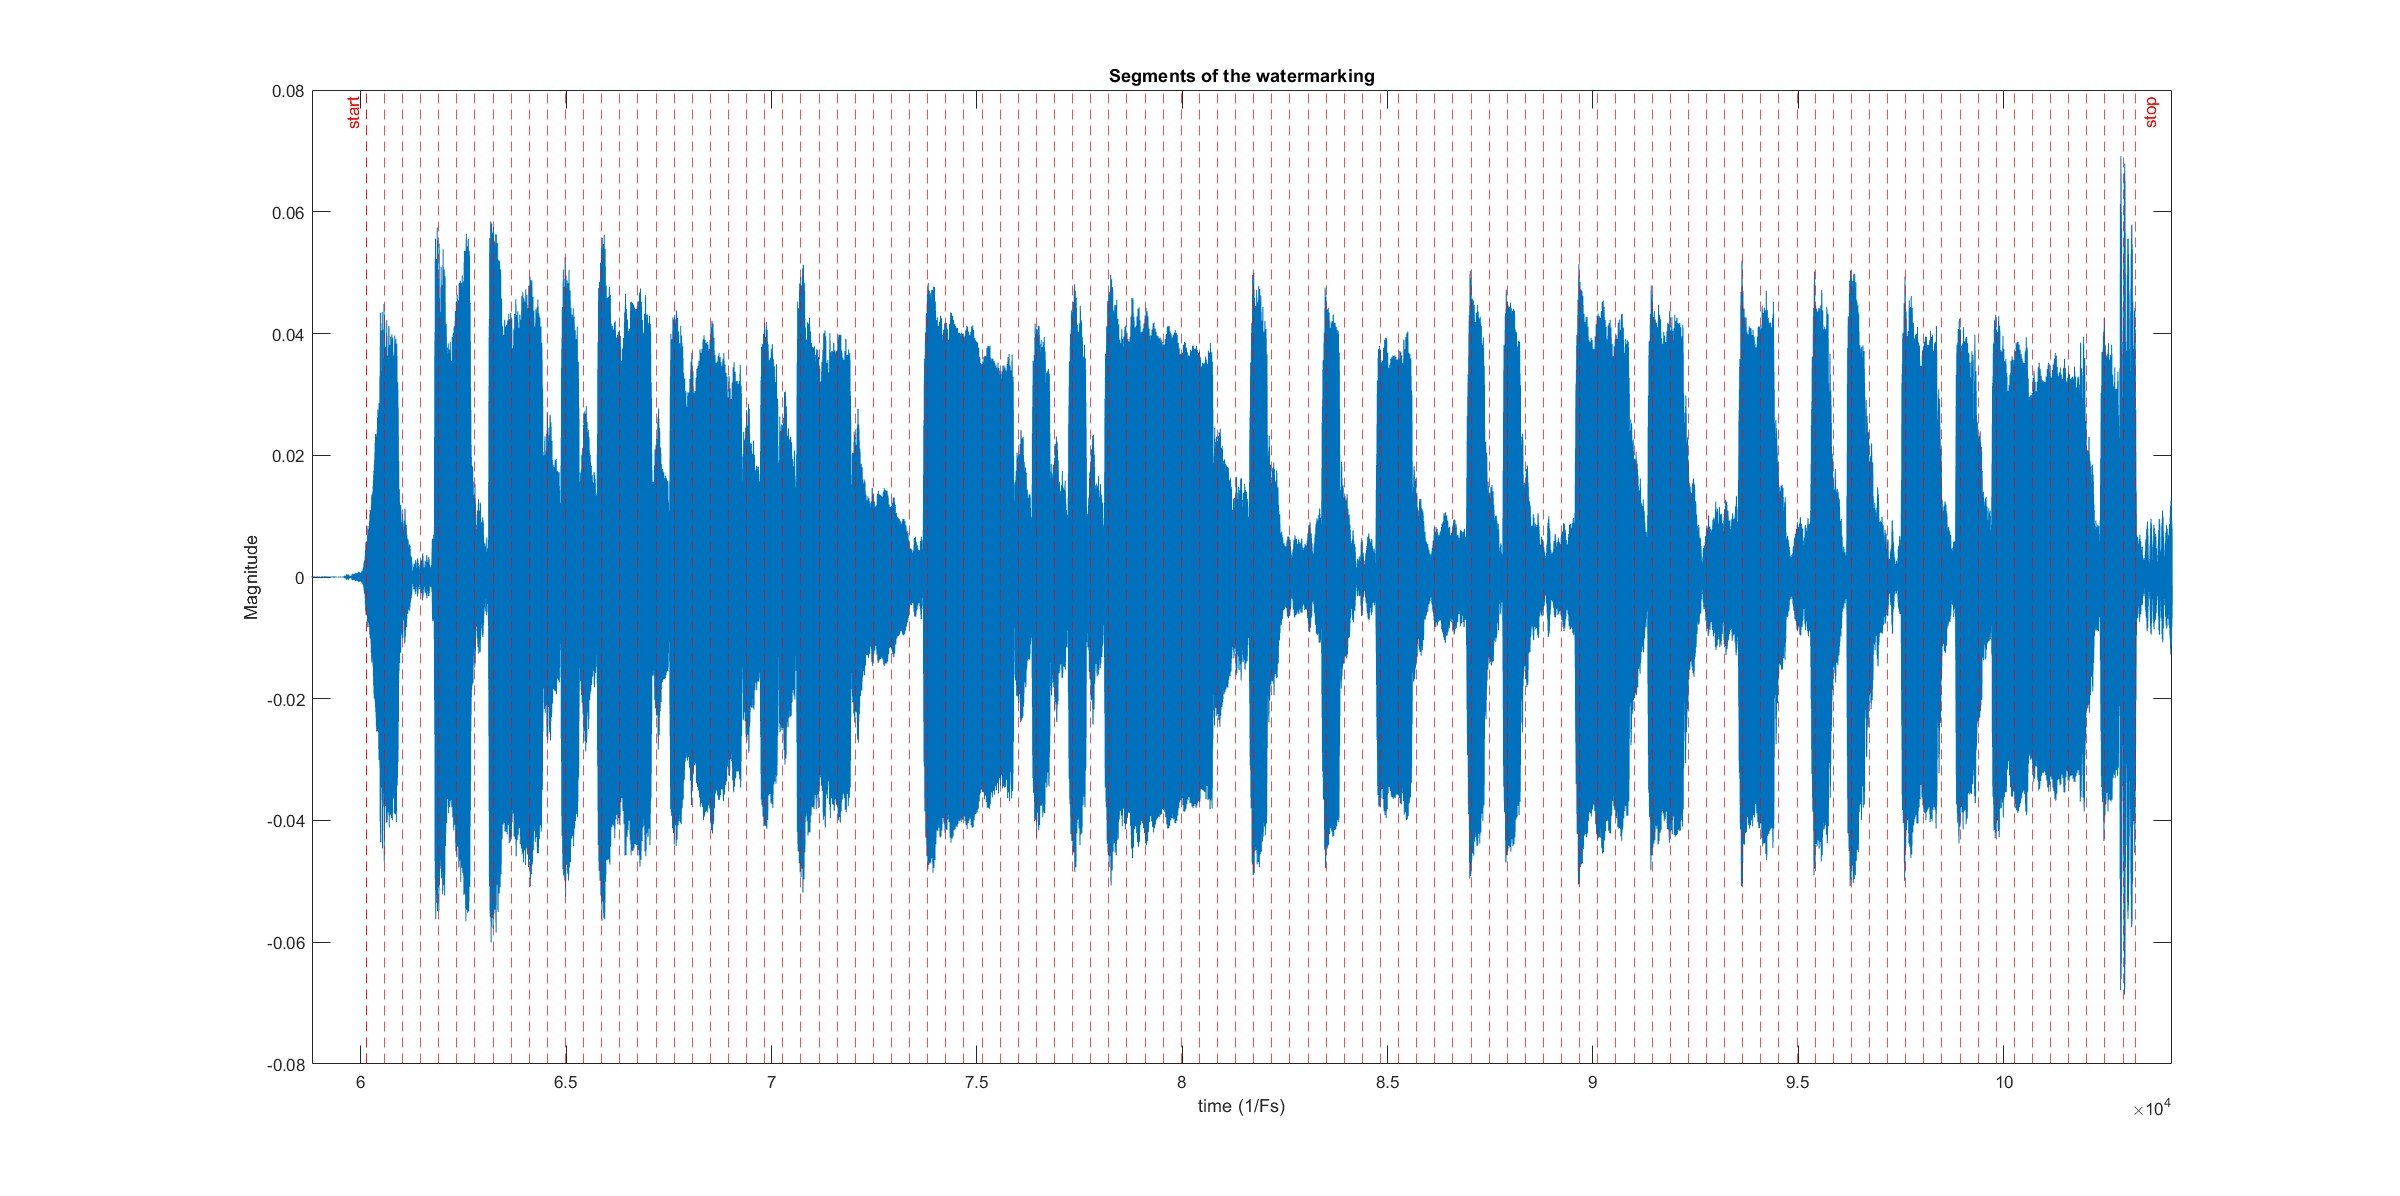
\includegraphics[width=\textwidth]{LiveAudioWatermarking/images/sgments.jpg}
    \caption{Segments representing the tones in the audio sample.}
    \label{fig:segments}
\end{figure}

Before assessing the segments, it is essential to establish a threshold that allows to determine whether a frequency (and consequently a symbol) is present within a segment or not. 
To accomplish this objective, an analysis with Goertzel algorithm is made, the result are showed in figure \ref{fig:goertzel}. 
\begin{figure}[H]
    \centering
    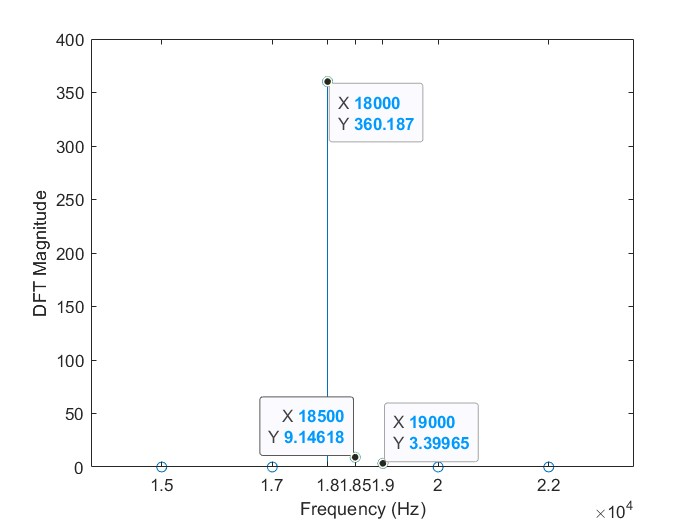
\includegraphics[width=0.8\linewidth]{LiveAudioWatermarking/images/Goertzel-full.jpg}
    \caption{Analysis with Goertzel Algorithm}
    \label{fig:goertzel}
\end{figure}

The values highlighted in the figures changes in every recording, therefore the needed threshold depends on the energy of the signal, that is not guaranteed to be constant throughout the sample (i.e. within a segment, one may find a magnitude different from that in another segment representing the same symbol).
A simplistic approach has been adopted: Assuming the frequency is distributed across all segments, one can calculate a sort of average energy by dividing the magnitude of the frequency in the entire signal by the total number of segments. This value can then be adjusted as needed (since each track is unique) by simply multiplying it by a constant.
In the context of this specific scenario, the number of segments has been computed. Consequently, the mean value is computed by dividing the overall signal magnitude by this quantity. 
\[Thr_{symb} = k\times\frac{ABS(goertzel(f_{symb}))}{N_{seg}}\]
In light of the aforementioned reasons the determination of \textit{k}, in this project,  is empirical, the attributed value is 0.8. For the start and stop bit, since the energy is cointained in a single segment, the chosen threshold is half of the total magnitude.
In figure \ref{fig:symbols} the results of the Goertzel algorithm applied to the segments are depicted. Specifically, an analysis per symbol is presented. From the represented values, the recognition mechanism of each one is easily discernible: each magnitude is compared to its threshold and the magnitudes of the other symbols, yielding the result readily.
\begin{figure}[H]
    \centering
    \begin{subfigure}{0.48\textwidth}
    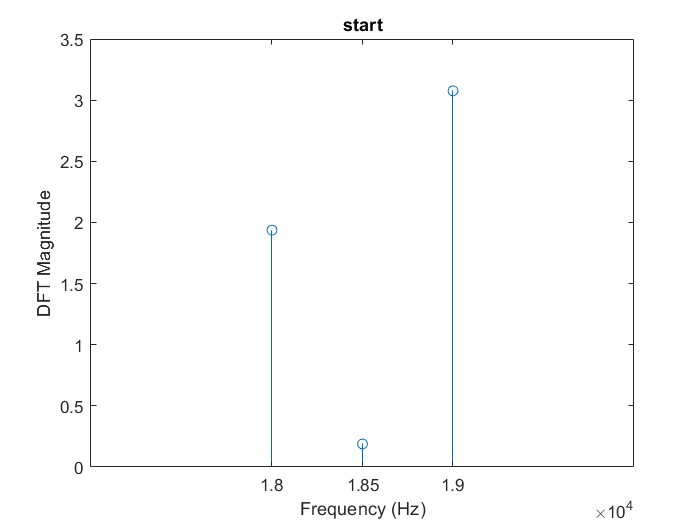
\includegraphics[width=\textwidth]{LiveAudioWatermarking/images/start_bit.jpg}
    \caption{}
    \label{}
    \end{subfigure}%
    \hfill
     \begin{subfigure}{0.48\textwidth}
    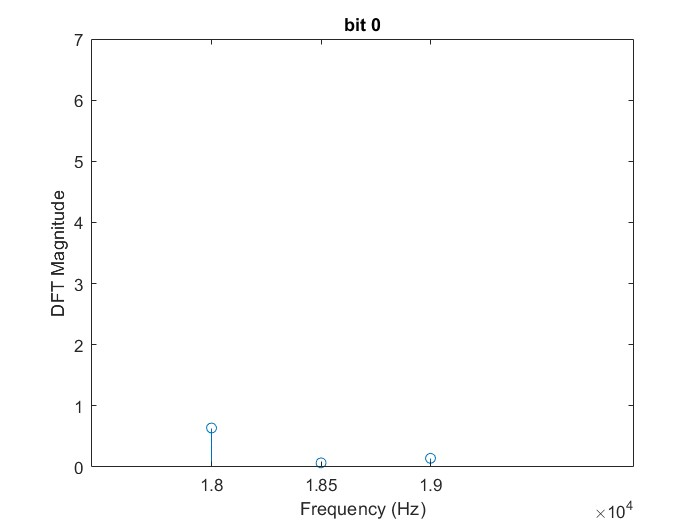
\includegraphics[width=\textwidth]{LiveAudioWatermarking/images/bit0.jpg}
    \caption{}
    \label{}
    \end{subfigure}\\
        \begin{subfigure}{0.48\textwidth}
    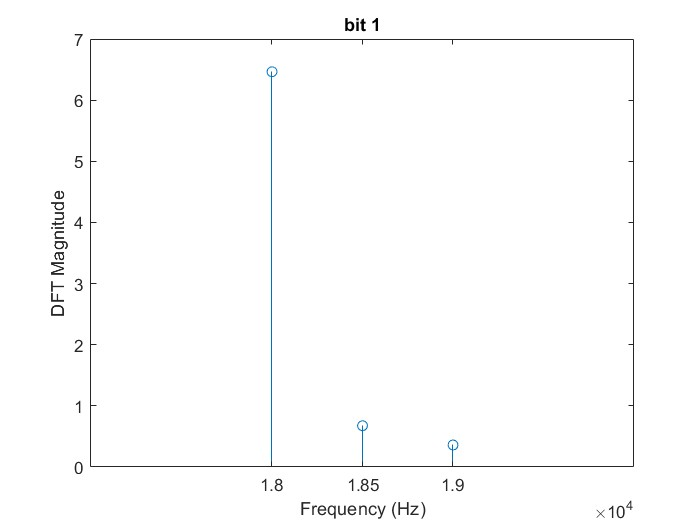
\includegraphics[width=\textwidth]{LiveAudioWatermarking/images/bit1.jpg}
    \caption{}
    \label{}
    \end{subfigure}%
    \hfill
     \begin{subfigure}{0.48\textwidth}
    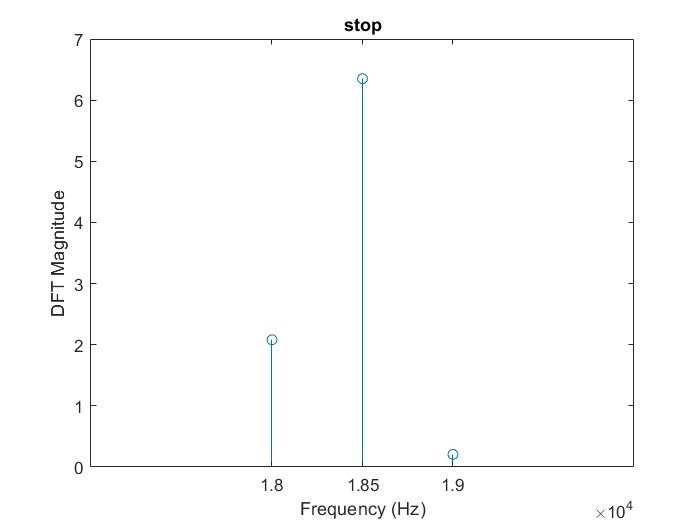
\includegraphics[width=\textwidth]{LiveAudioWatermarking/images/stop_bit.jpg}
    \caption{}
    \label{}
    \end{subfigure}
    \caption{Frequency encoding of the symbols}
    \label{fig:symbols}
\end{figure}
In this case the received binary string is "9BAEF5C3EAFE898A3B194D7D", that can be represented as a Unicode string, but the encrypted output manifests as a sequence of seemingly random characters, devoid of any meaning.
At this stage, the solution to retrieve the data, is to employ the designated decryption tool. The tool is invoked with Matlab's command \texttt{system()}, passing as arguments the binary string (in binary representation) and the previously defined encryption key, the output is saved in case further operation are needed.

In this experiment the resulting string still contains unintelligible characters: those are the latitude and longitude values of the GPS location, that needs to be converted into a IEEE 754 float representation.

Finally the watermark is successfully extracted and the information are in human readable form.

\section{Known Issues}
The work described in the preceding sections was conducted in a controlled environment, with the following characteristics:
\begin{itemize}
    \item \textbf{The room was not noisy}, even if the audible noise (e.g. air condition, chatter etc), does not have impact on the selected frequency and it is filtered.
    \item \textbf{The watermarking device was situated a few centimeters away from the microphone}, to guarantee a sufficient power to detect the signal
    \item  \textbf{The transmission was kept short}, since the watermark is extracted with simple signal processing technique
    \item  \textbf{The bitrate was set to an already verified value}, since the tone length was set to 10 ms the bitrate is 100 bit/s, that is sufficient considering recordings of a minimum duration of few seconds, but relatively slow considering the sampling frequency.
\end{itemize}

This characteristics stem from the issues encountered during the experimental trials, which are:
\begin{itemize}
    \item \textbf{Non-linearity of the smartphone's speaker:} when playing the audio watermark, sudden frequency shifts occurs. In an ideal case, this should not result in any noise coming from the device, but in this implementation,  a \textit{"crackling"} sound is audible. This sound is below the designed frequencies, indeed it is removed by the band pass filter. 
    At the current state of the project, the source of this issue is not totally certain but possible improvement are discussed in the \textit{Future Work} section.
    \item \textbf{Limiting range of near-ultrasound frequencies tones:} as previously discussed the implementation has been pursued with devices that are suitable for the selected frequency range, therefore the functionality is not guaranteed on other devices (e.g. Iphone). This issue affects also the recognition of tones with the cross correlation, since the tones have similar frequency.
    \item \textbf{Possible instability of the developed software:} the developed application is a prototype, therefore the performance and correctness of the code is not guaranteed: some delays have been noticed in long transmission (e.g. irregular tone duration) that can lead to misinterpretation of the symbols, because of misalignment of the symbol's window.
    Furthermore, with the current software, setting a lower duration of the tone may result in a tone skip, or no output at all.\\
    The output of the first tone has some latency, resulting in having a lower magnitude with respect to the others.
    The script for decoding the watermark may need \textit{"ad-hoc"} tuning for retrieving sample in some condition ( e.g. changing the threshold, failing to detect start/stop tone).

    
\end{itemize}

\section{Future Work}
%Adding a section about how to improve the project is not mandatory but it is useful to show that you actually understood the topics of the project and have ideas for improvements.%
Considering the issues listed in the previous section, we can outline some potential improvements to be addressed as future work. 
The first improvement consist into a better quality of the watermarked signal: starting from the software, an experience app developer or a more in depth research endeavor, can make application transmit a more sharper signal, solving the issues related to timing performances. Also, alternative approaches to the chosen modulation technique can improve both the density of the watermark and its robustness, for example APSK (Amplitude and phase-shift keying) allows for a lower bit error rate, at the cost of the increased complexity in the development of a transmitting e receiving software.
Regarding the hardware, utilizing an external device such as a mini speaker equipped with ultrasonic transducers, connected to the smartphone's audio interface (e.g., audio jack, Bluetooth, USB-C), could significantly enhance the signal. This external device has the capability to reproduce '0' and '1' bits at a higher frequency, ensuring superior performance and potentially amplified power. Additionally, the transmitted signal can be split into stereo channels, allocating the right channel for one bit symbol and the left channel for the other, further optimizing the transmission process. Furthermore, the ultrasonic transducers, being capable of working in ultrasound frequency, open up the possibility of injecting a signal into frequencies near ultrasound, leveraging the intrinsic nonlinearities of the MEMS microphones.

Another area of enhancement of this work is to developed a better post processing analysis, exploiting more complex and advanced technique used in modern digital signal processing.
An additional feature that can be developed is live processing, making the less experienced users able to easily check the presence of the watermark and its content.

Regarding the data to be embedded in the signal, there exists a plethora of possibilities. Unique device identification codes, such as IMEI numbers, can be retrieved. Additionally, a wide array of sensors available on any smartphone offers diverse choices for data incorporation.